\documentclass[conference]{IEEEtran}
\IEEEoverridecommandlockouts
\usepackage{cite}
\usepackage{amsmath,amssymb,amsfonts}
\usepackage{algorithm}
\usepackage{algpseudocode}
\usepackage{graphicx}
\usepackage{textcomp}
\usepackage{xcolor}
\usepackage{tikz}
\usetikzlibrary{positioning,arrows.meta}
\usepackage{booktabs}
\usepackage{array}
\usepackage{balance}
\usepackage{listings}

\def\BibTeX{{\rm B\kern-.05em{\sc i\kern-.025em b}\kern-.08em
    T\kern-.1667em\lower.7ex\hbox{E}\kern-.125emX}}

\begin{document}

\title{Local AI Meeting Intelligence Using Parallel LLM Extraction and Hybrid Retrieval}

\author{\IEEEauthorblockN{Sanjay Nesan J}
\IEEEauthorblockA{Division of Data Science and Cyber Security\\
Karunya Institute of Technology and Sciences\\
Coimbatore, India\\
sanjaynesan@karunya.edu.in}
\and
\IEEEauthorblockN{Dr. Revathi B.S.}
\IEEEauthorblockA{Division of Data Science and Cyber Security\\
Karunya Institute of Technology and Sciences\\
Coimbatore, India\\
revathi@karunya.edu.in}}

\maketitle

% [ADDED/REVISED] Abstract and index terms; reports only measured values and their limitations.
\begin{abstract}
Meeting transcripts contain decisions, assignments, risks, and unresolved questions, yet extracting these items can expose sensitive organizational data and produce unsupported statements. This paper presents a locally processed meeting-intelligence prototype combining speech transcription, parallel structured extraction with Qwen2.5-7B, lexical transcript-overlap checks, keyword search, dense retrieval, and Reciprocal Rank Fusion (RRF). The extraction benchmark on two manually annotated meetings reports a macro F1 score of 0.6534 across decisions, action items, risks, and unanswered questions. A separate audit of three stored meeting outputs reports that 48 of 51 extracted items pass a 20\% lexical-overlap threshold; this heuristic is not a human-validated factuality measure. In one sequential-versus-parallel timing run, wall-clock latency decreased from 490,289 ms to 306,385 ms (37.51\%), but four parallel extraction stages failed, so the comparison does not establish equivalent completed work. Retrieval relevance was not measured because no labeled query set was available and the recorded RAG timing used a MongoDB fallback. The results describe a preliminary systems contribution and motivate broader evaluation.
\end{abstract}

\begin{IEEEkeywords}
meeting intelligence, speech recognition, large language models, information extraction, hybrid retrieval, transcript grounding, local inference.
\end{IEEEkeywords}

% [REVISED] Research questions and contributions narrowed to measured evidence and implementation scope.
\section{Introduction}

Organizations increasingly accumulate meeting recordings whose decisions, action items, and discussion context are difficult to preserve and retrieve through manual note-taking. Conventional meeting records often capture only selected points and provide limited support for locating information across a growing collection of recordings. Automated meeting-intelligence systems can address this problem by converting spoken discussions into searchable and structured information, but the resulting pipeline must handle speech recognition, speaker attribution, information extraction, storage, and retrieval as a connected process.

Existing approaches often focus on individual components such as speech processing, meeting summarization, structured extraction, or information retrieval rather than their integration into a unified meeting-memory pipeline. Speech recognition and diarization can produce transcripts with speaker information, while large language models (LLMs) can transform transcripts into summaries and structured information. However, extracting multiple meeting dimensions independently introduces consistency and validation requirements, and retrieving information from long-term meeting collections requires both lexical and semantic matching. These challenges become more important when meeting content contains sensitive organizational information that cannot be routed through third-party cloud inference services.

This work addresses these challenges through a modular meeting-intelligence architecture designed for local processing. After model provisioning, meeting audio, transcripts, embeddings, and derived intelligence are processed locally without external inference APIs. The pipeline combines speech-to-text and speaker diarization with parallel LLM-based extraction, schema validation, retry handling, transcript grounding, incremental embedding, hybrid retrieval, and retrieval-augmented generation (RAG). The resulting structured meeting memory supports both targeted retrieval and conversational access to previously processed meetings.

The study investigates three questions. \textbf{RQ1:} What wall-clock latency was observed for sequential and parallel extraction, and how complete were the parallel stages? \textbf{RQ2:} Does hybrid keyword and dense-vector retrieval improve meeting-memory retrieval quality over either method alone? This remains future work because relevance labels are unavailable. \textbf{RQ3:} How often do extracted items pass the implemented lexical-overlap check, and how well does that check correspond to human judgments? The current audit addresses only the first part; human validation remains future work.

The contributions are systems-oriented: (1) integration of local speech processing, structured extraction, transcript storage, and search; (2) a nine-stage parallel extraction implementation with stage-specific validation and normalization; (3) a preliminary two-meeting extraction evaluation and a separate lexical-overlap audit, with limitations stated; and (4) implementation of an RRF hybrid retrieval path, whose retrieval effectiveness remains to be measured. After model provisioning, inference and indexing are designed to run locally; this describes the deployment architecture and is not a broader security guarantee.

The remainder of this paper presents related work and the research gap, describes the proposed system and core algorithms, details the experimental methodology, reports the results and discussion, and concludes with the limitations and conclusion.

 

% [REVISED] Citations corrected, MeetingBank limited to summarization, and system novelty positioned accurately.
\section{Related Work and Research Gap}

\subsubsection{Speech Recognition and Speaker Diarization}

Automatic speech recognition (ASR) has progressed through large-scale weakly supervised training. Whisper provides a multilingual speech-recognition model \cite{whisper}, while WhisperX adds time-aligned transcription and related processing \cite{whisperx}. Speaker diarization systems such as pyannote.audio identify speaker turns \cite{pyannote}. These components provide an input layer for meeting intelligence; they do not by themselves represent decisions or other meeting knowledge.

\subsubsection{Meeting Summarization and Structured Extraction}

Meeting summarization benchmarks include QMSum \cite{qmsum} and MeetingBank \cite{meetingbank}; these works are cited as summarization resources, not as evidence of action-item extraction. Automatic minuting has also been studied in the AutoMin shared task \cite{automin}. Independent extraction of multiple information categories introduces consistency, schema-conformance, and unsupported-content risks. Structured-output techniques can support downstream processing \cite{jsonschema}, but meeting systems still require validation connecting generated fields to source transcripts.

\subsubsection{Retrieval-Augmented Generation and Hybrid Retrieval}

Retrieval-augmented generation combines retrieval with language-model generation \cite{rag}. Dense Passage Retrieval (DPR) is a neural dense-retrieval method \cite{dpr}. Lexical retrieval methods such as BM25 rank documents using term statistics \cite{bm25}, while the prototype's MongoDB keyword path is not asserted to be a BM25 implementation. Reciprocal Rank Fusion (RRF) combines ranked lists without requiring their raw scores to be comparable \cite{fusion}. The prototype implements an RRF path, but its relevance effectiveness has not yet been measured.

\subsubsection{Grounding and Hallucination Mitigation}

LLM-generated meeting information can contain unsupported statements. Hallucination surveys describe the challenges in detecting and evaluating such content \cite{halluc_survey}. SelfCheckGPT is one black-box hallucination-detection approach \cite{selfcheckgpt}, but it is not used in this prototype. Here, word overlap is only a lightweight audit signal and cannot establish semantic entailment or factual correctness.

\subsubsection{Research Gap and Positioning}

The reviewed work covers speech recognition, diarization, meeting summarization, structured extraction, retrieval, and grounding. This paper positions its contribution as an engineering integration of these established components for local meeting-memory workflows. It does not claim a new model architecture, retrieval algorithm, or measured retrieval-quality gain. A product-level comparison is outside the evidence reported here.

% [REVISED] Architecture text and screenshot captions describe the supplied implementation and image assets.
\section{Proposed System}

\subsubsection{System Architecture}
The proposed meeting-intelligence system converts recordings into structured and searchable meeting data through a modular processing pipeline. As shown in Fig.~\ref{fig:architecture}, audio or video is processed by speech recognition and speaker diarization. The speaker-attributed transcript is passed to a parallel LLM extraction layer. Outputs are schema-validated and normalized; a lexical-overlap check is applied to selected fields. Meeting content is indexed for semantic retrieval. At query time, keyword and dense-vector results can be fused using Reciprocal Rank Fusion (RRF) and supplied to the RAG component.

The architecture separates speech processing, extraction, validation, storage, and retrieval into independent stages. After model provisioning, the configured inference and indexing workflow is intended to run locally without external inference APIs.
\begin{figure}[t]
\centering
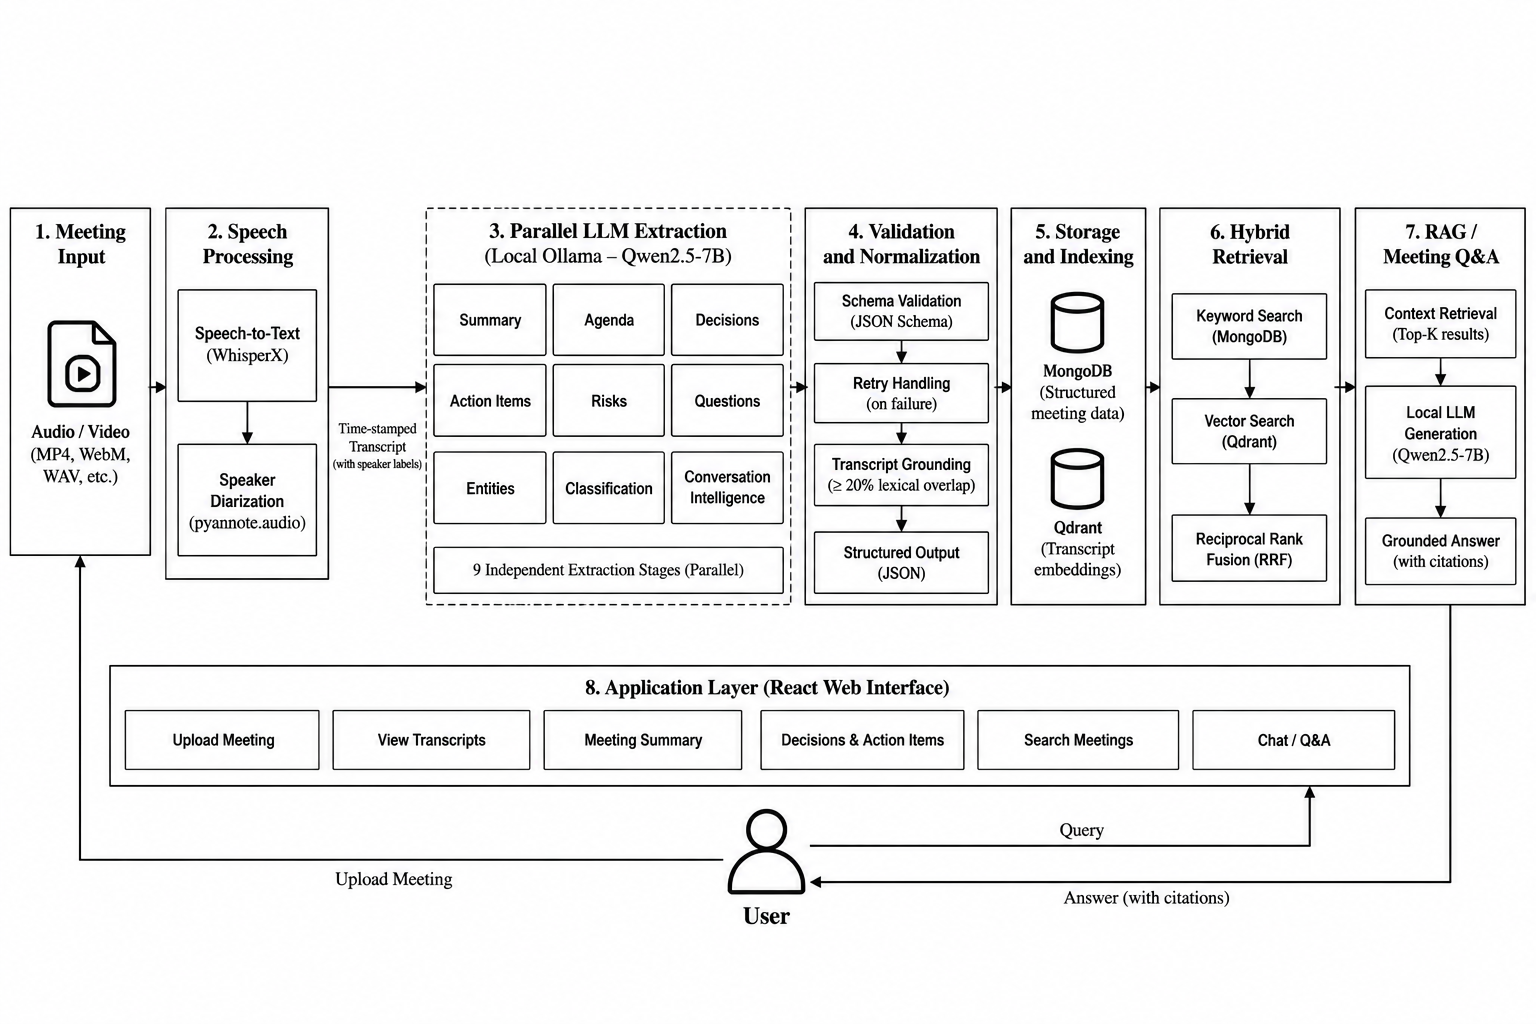
\includegraphics[width=\columnwidth]{architecture.png}
\caption{Architecture of the local meeting-intelligence pipeline, from recording ingestion and parallel extraction to indexed meeting memory and RRF-based retrieval.}
\label{fig:architecture}
\end{figure}

\subsubsection{Speech Processing and Speaker Alignment}
The first stage converts meeting audio or video into a time-aligned transcript using a locally hosted speech-recognition model. Speaker diarization is performed independently to identify speaker turns. The diarization segments and transcription segments are then aligned using their temporal overlap so that each transcript segment can be associated with the most strongly overlapping speaker segment.

The resulting representation preserves both textual content and speaker attribution. This information is important for downstream extraction because decisions, action items, questions, and statements may need to be associated with the participant who produced them. The system therefore treats speaker attribution as part of the meeting-memory representation rather than as an independent visualization feature.

\subsubsection{Parallel Multi-Stage LLM Extraction}
The speaker-attributed transcript is processed by a parallel extraction layer based on a locally hosted LLM. Instead of requesting every meeting attribute through a single large extraction operation, the system divides the task into nine independently executed stages:
\begin{enumerate}
    \item summary, 
    \item agenda, 
    \item decisions, 
    \item action items, 
    \item risks, 
    \item questions, 
    \item entities, 
    \item meeting classification, and 
    \item conversational intelligence. 
\end{enumerate}
Each stage uses a task-specific prompt and produces structured output according to a predefined schema. Independent stages can execute concurrently, reducing dependence between extraction tasks. The resulting outputs are passed through schema validation and normalization before being combined into the final meeting representation.

\subsubsection{Validation, Normalization, and Transcript Grounding}
The extraction layer includes validation mechanisms to prevent malformed or incomplete model output from propagating into the meeting database. Schema validation checks the expected structure and field types, while retry handling provides an additional inference attempt when a stage fails validation. A normalization stage standardizes extracted values such as priorities and deadlines before the outputs are stored.

The system applies a lexical-overlap heuristic to selected extracted information. For each item, words longer than three characters are compared with the entire source transcript; an item passes when at least 20\% of those words occur anywhere in that transcript. This is an audit signal, not a semantic entailment test, and whole-transcript matching can allow broadly on-topic text to pass. Runtime behavior varies by field: some validators log a failed check while retaining the item, whereas risk validation can omit items that fail.

\subsubsection{Incremental Embedding and Hybrid Retrieval}
Processed meeting content is transformed into embedding vectors and stored in a vector index for semantic retrieval. The indexing process uses content-addressable identifiers to avoid unnecessary duplication when previously processed content is encountered again. In parallel, structured meeting information remains available for keyword-based retrieval.
For a user query, the system obtains ranked results from both keyword and dense-vector retrieval. The two ranked lists are combined using RRF, which assigns higher combined scores to documents appearing near the top of multiple retrieval lists. The resulting ranked context is passed to the RAG layer, which generates an answer using the retrieved meeting information rather than relying only on the language model's internal knowledge.

For a result $d$, the implementation uses
\begin{equation}
\operatorname{RRF}(d)=\sum_{i=1}^{m}\frac{1}{k+\operatorname{rank}_{i}(d)},\quad k=60,
\end{equation}
where $m$ is the number of ranked lists and a result absent from a list contributes no term. MongoDB keyword ranking is a separate additive field-weight score: each case-insensitive regular-expression match contributes the configured weight for that field (e.g., decisions: 10; action-item task/description: 9; summaries/keywords: 8; transcript: 3). It is not BM25. The current MongoDB path ranks meeting records, while Qdrant produces transcript chunks; the RRF implementation uses meeting IDs when available to fuse results. Any relevance evaluation must therefore use the common meeting-level ranking unit, or first add a chunk-level keyword baseline.

\subsubsection{Meeting Memory and RAG Interaction}
The final meeting representation contains both structured fields and searchable content. Structured fields support operations such as filtering and direct retrieval of decisions or action items, while embeddings support semantic search across meeting content. The hybrid retrieval layer therefore provides complementary lexical and semantic access to the same organizational memory.

For conversational queries, the retrieved evidence is supplied to the RAG component as contextual information. This design enables users to ask questions about previously processed meetings while maintaining a direct retrieval path to the underlying meeting records.

\subsubsection{Application Interface}
Fig.~\ref{fig:dashboard} shows the meeting analytics dashboard. Fig.~\ref{fig:ragui} presents the meeting-memory question-answering interface. Fig.~\ref{fig:analytics} displays meeting analytics and search controls, while Fig.~\ref{fig:details} shows extracted action items, entities, and question panels.
\begin{figure}[t]
\centering
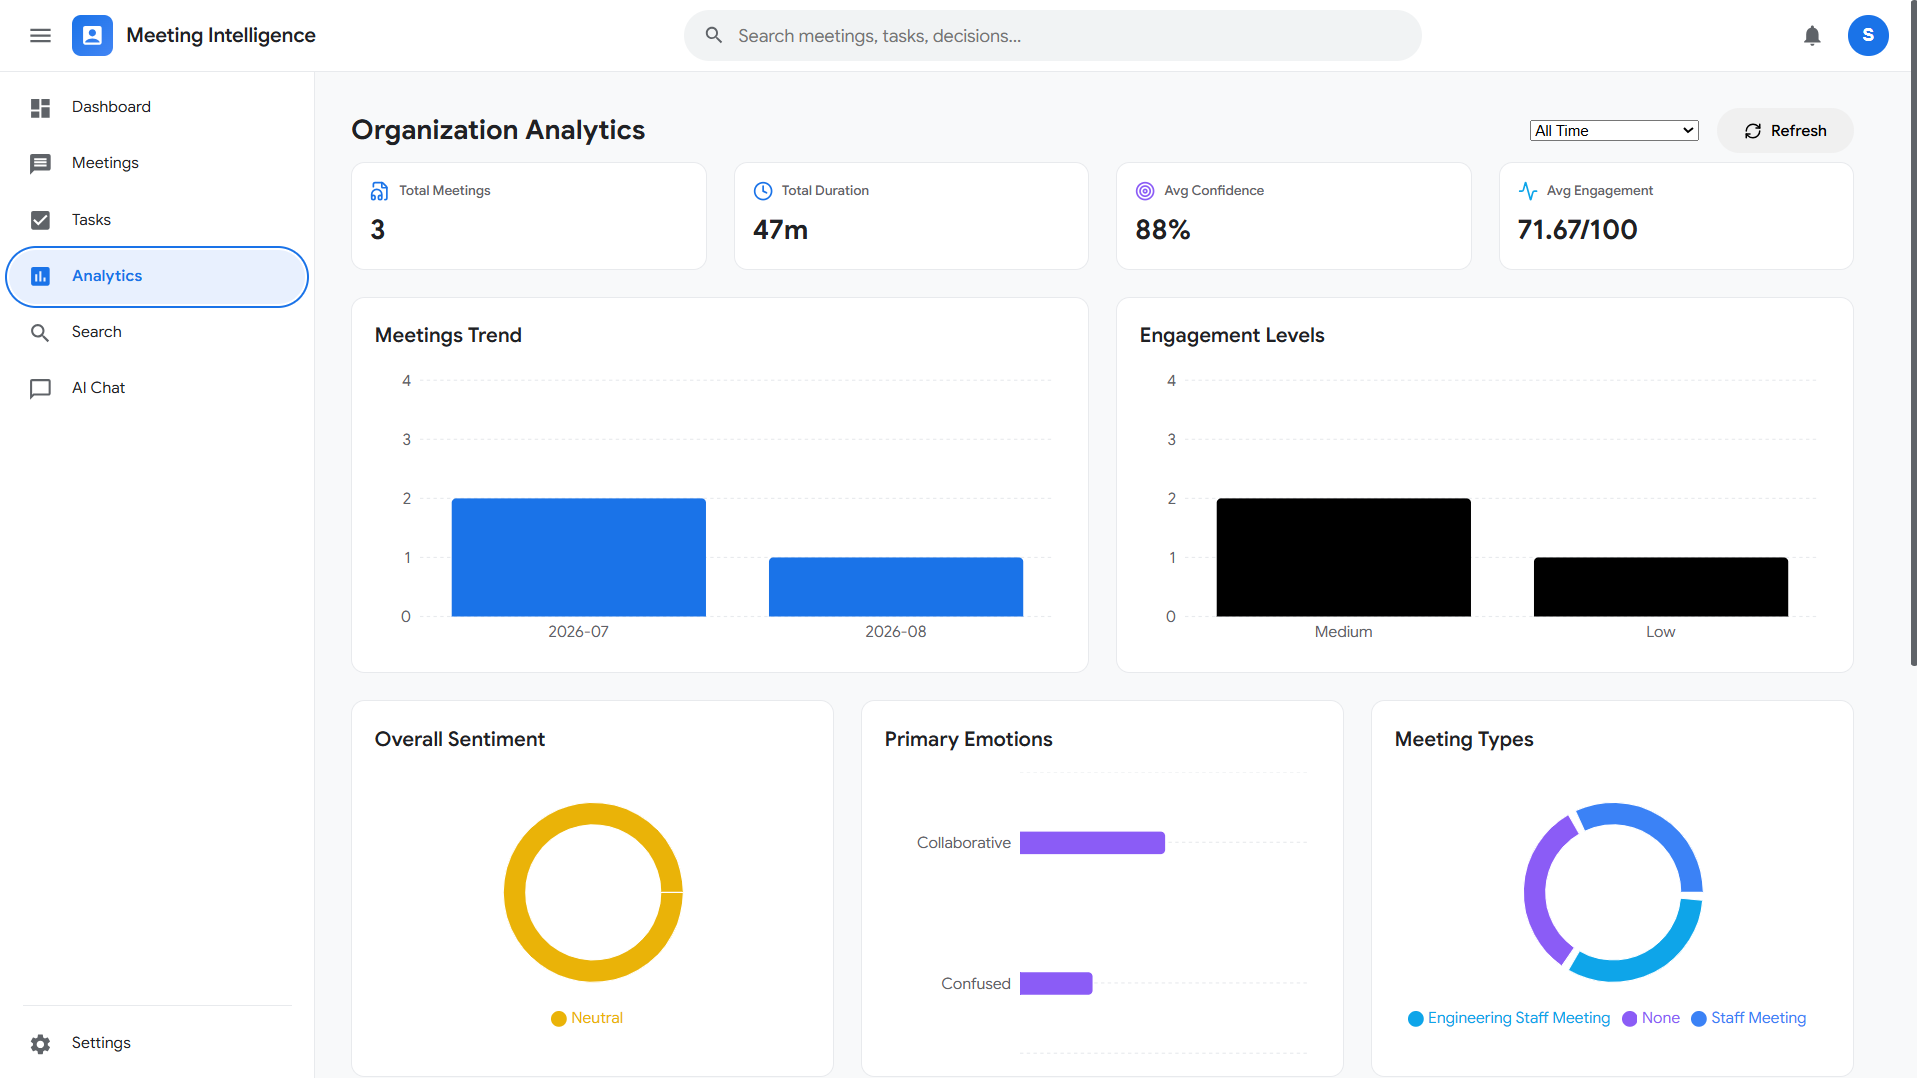
\includegraphics[width=\columnwidth]{fig2.png}
\caption{Meeting analytics dashboard showing summary metrics and visualized meeting statistics.}
\label{fig:dashboard}
\end{figure}
\begin{figure}[t]
\centering
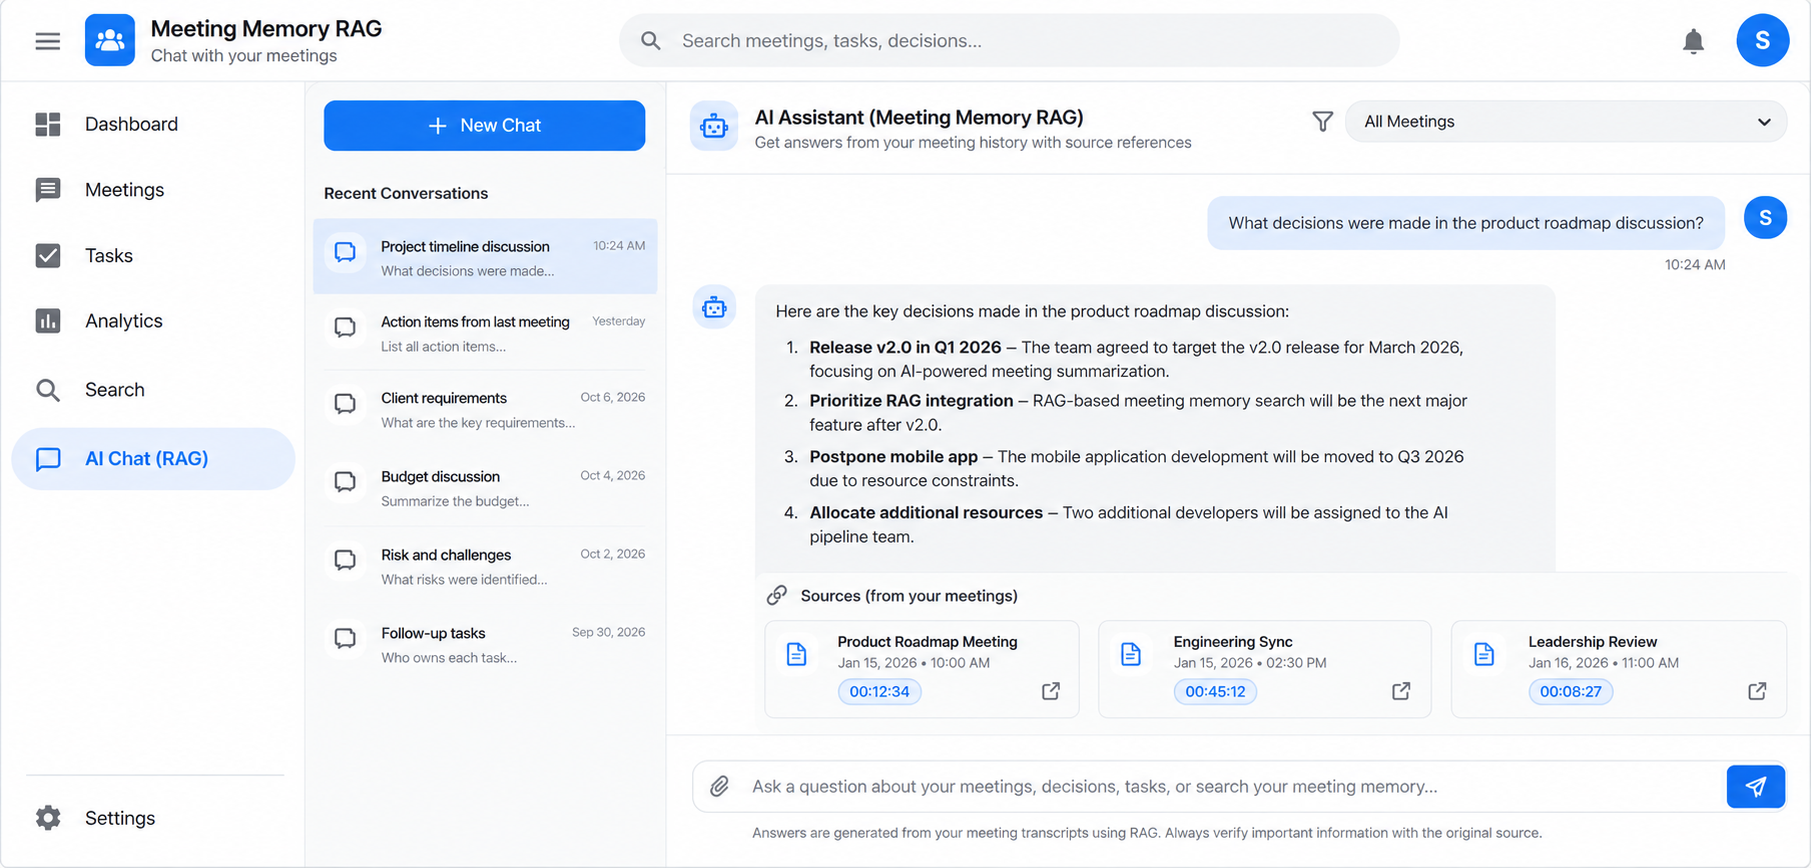
\includegraphics[width=\columnwidth]{fig3.png}
\caption{Meeting-memory question-answering interface displaying a user query and retrieved response.}
\label{fig:ragui}
\end{figure}
\begin{figure}[t]
\centering
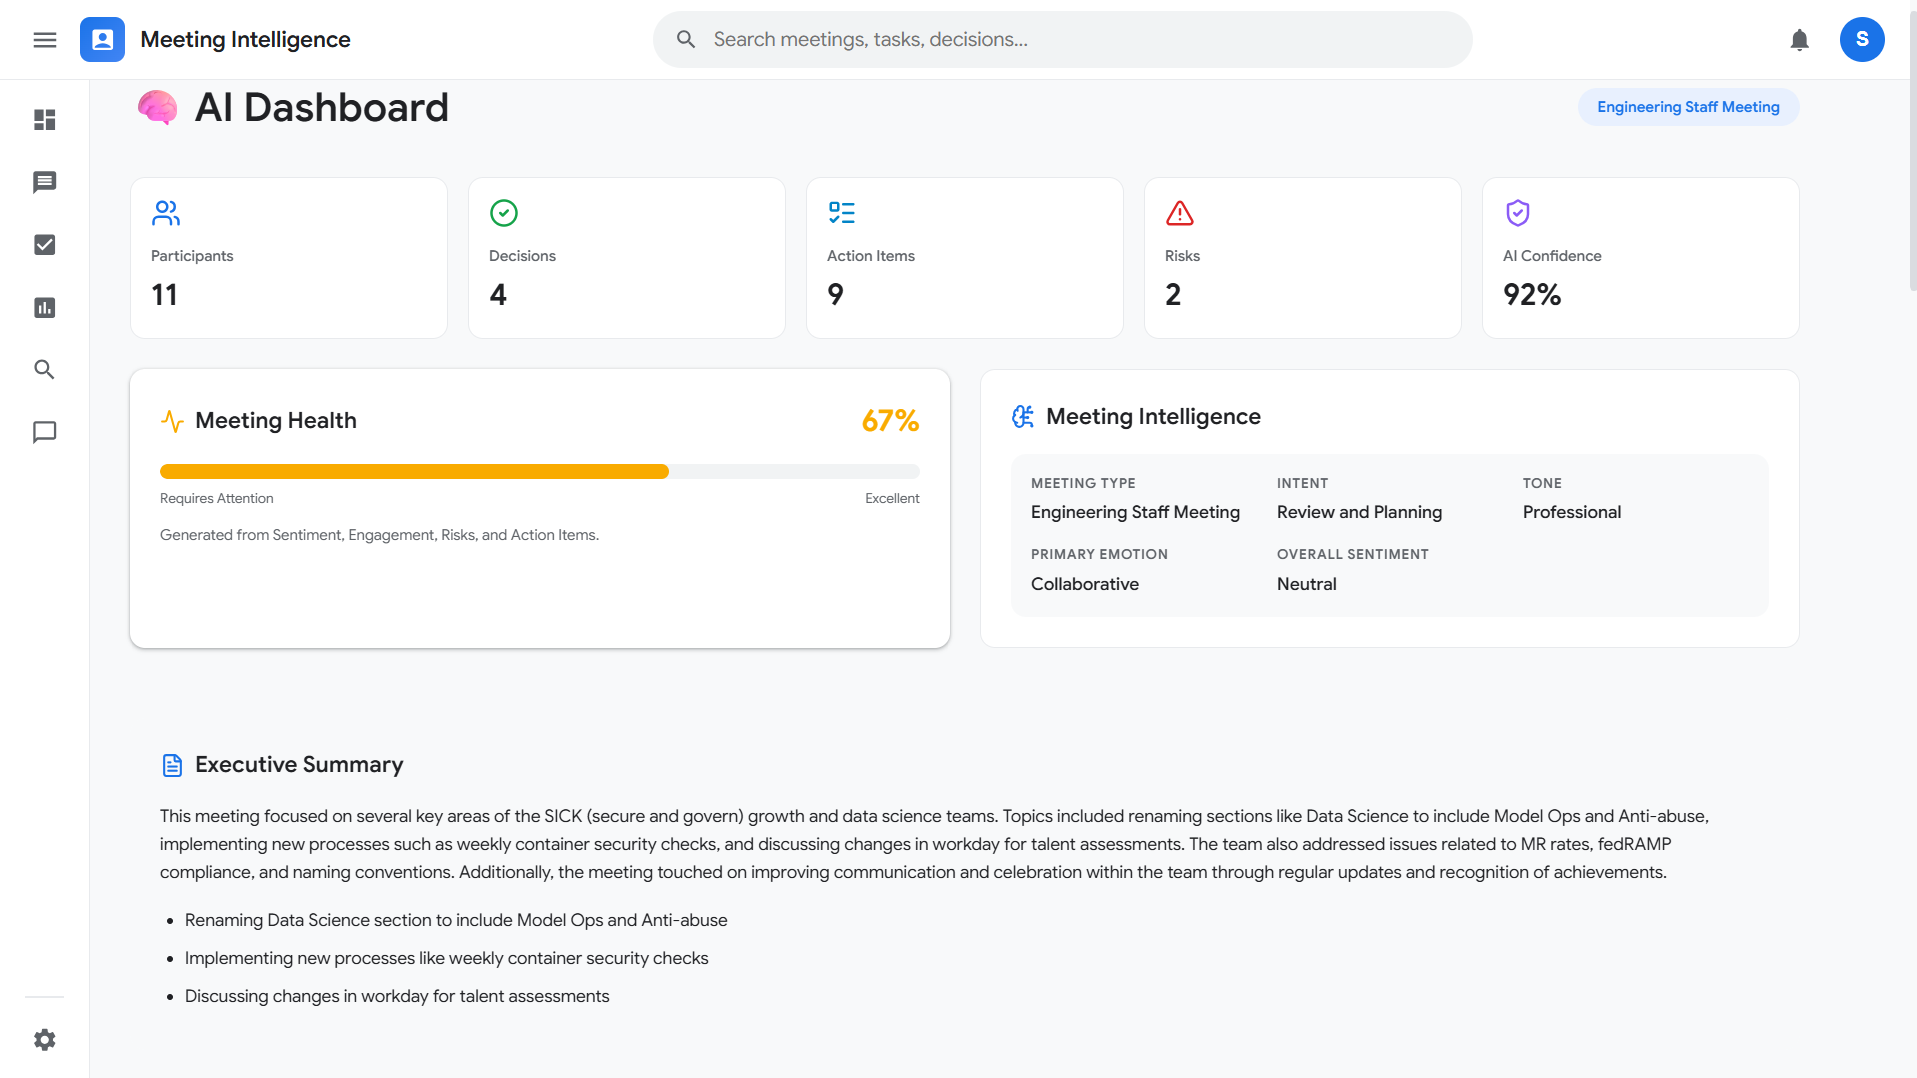
\includegraphics[width=\columnwidth]{fig4.png}
\caption{Meeting analytics and search interface with structured meeting indicators and summary content.}
\label{fig:analytics}
\end{figure}
\begin{figure}[t]
\centering
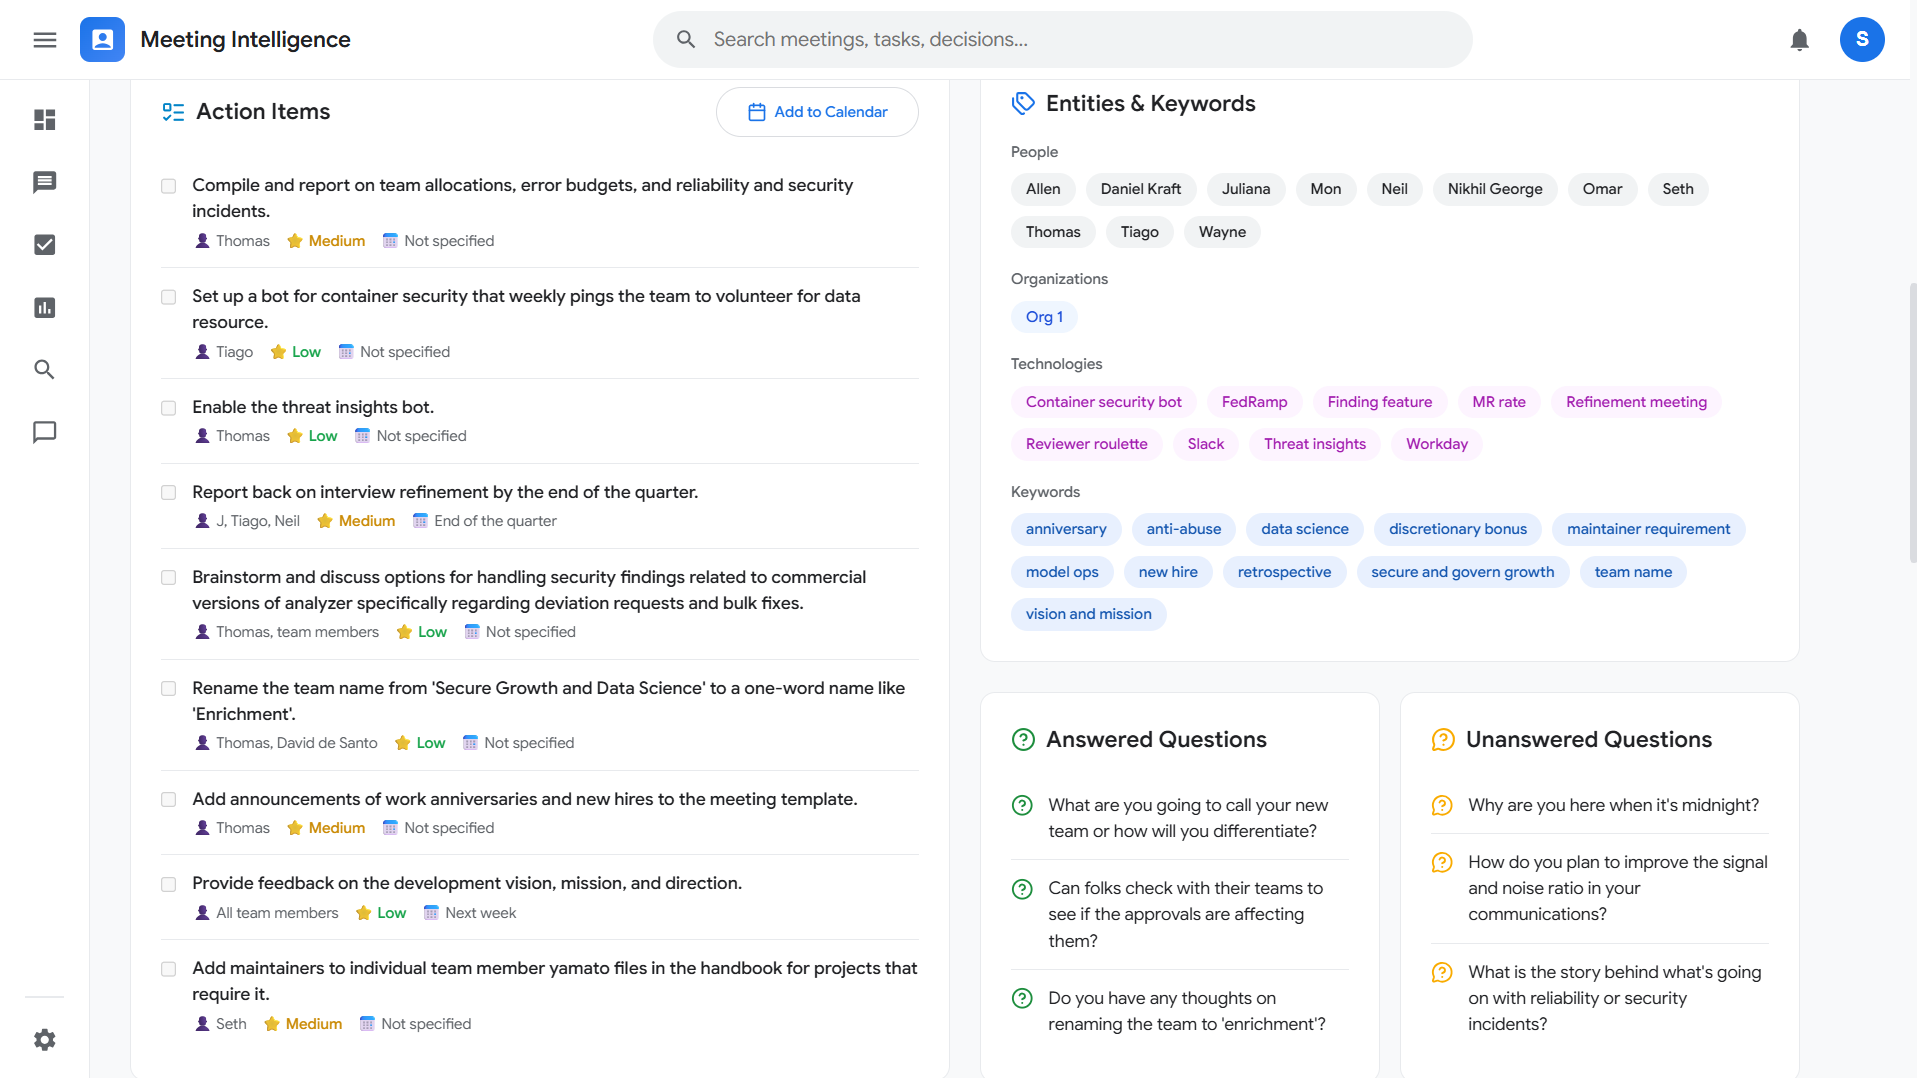
\includegraphics[width=\columnwidth]{fig5.png}
\caption{Meeting detail interface presenting extracted action items, entities, and question categories.}
\label{fig:details}
\end{figure}

% [ADDED/REVISED] Dataset scopes, measured configurations, baseline plans, retrieval protocol, and grounding validation design.
\section{Experimental Methodology}

\subsection{Experimental Setup}
The extraction and timing benchmark used Ollama model tag \texttt{qwen2.5:7b} \cite{qwen25}, temperature 0, an 8,192-token context, and a 24,000-character transcript limit. The reported workstation had a 12th-generation Intel Core i5-12450H CPU, 16~GB RAM, and an NVIDIA RTX~3050 Laptop GPU with 4~GB reported memory. The installed model is listed as 4.7~GB, but its quantization and CPU/GPU offload allocation were not recorded. Nomic Embed \cite{nomic} was configured for 768-dimensional embeddings. The timing comparison was one run (n=1); its log identifies the input as the largest database transcript. The available inventory maps that record to Sec Growth DataScience (4,647 words, 24,310 characters), although the timing log does not preserve its ID. The raw transcript exceeds the configured limit by 310 characters. The timing log's 24,029-character input count does not match the configured 24,000-character limit. Ollama parallelism/model limits, retry attempts, worker limits, and batch size were not recorded, limiting reproducibility.

\subsection{Evaluation Corpus}
The system inventory contains three meetings totaling 2,858.39~s (47.64~min) and 7,987 transcript words. The extraction-quality benchmark uses two of them: ``Effective Meetings: Simulated Exercise for Chairing & Minute Taking'' (2,598 words; 849.61~s) and ``SICK - Secure and Govern Growth and Data Science Team Meeting'' (4,647 words; 1,743.47~s), totaling 7,245 words and 2,593.08~s. The Tamil-audio-labeled record (742 words; 265.31~s) is excluded from extraction accuracy; its inventory language field is ``en'', so its spoken language is unverified. The separate lexical-overlap audit covers all three saved outputs and 51 items. The inventory did not record speaker counts, domain labels, or acoustic conditions; these are shown as NR (not recorded) in Table~\ref{tab:corpus}.

\begin{table}[t]
\caption{Three-Meeting Evaluation Inventory}
\label{tab:corpus}
\centering
\scriptsize
\begin{tabular}{@{}lrrrrll@{}}
\toprule
\textbf{ID} & \textbf{Duration} & \textbf{Words} & \textbf{Spk.} & \textbf{Domain} & \textbf{Lang.} & \textbf{Acoustics} \\
\midrule
Tamil audio & 265.31 & 742 & NR & NR & en* & NR \\
Sec Growth & 1,743.47 & 4,647 & NR & NR & en & NR \\
Effective Meetings & 849.61 & 2,598 & NR & NR & en & NR \\
\bottomrule
\end{tabular}
\end{table}
\par\noindent *The record title says ``Tamil audio,'' while its stored language field is English; the spoken language is not established by this inventory.

\subsection{Extraction Metrics and Baselines}
The two reference files contain 37 manually annotated items in total. The annotation records do not document annotator count, annotator identity, or detailed guidelines, and no independent adjudication is reported. Predictions are processed in order and greedily matched one-to-one to the highest-Jaccard unused reference item when token Jaccard similarity is at least 0.5. This matching rule can penalize paraphrases and is order-dependent; no semantic or human spot-check of borderline matches is available. Precision, recall, and F1 are calculated per category, with category metrics micro-aggregated across the two meetings and macro-averaged across the four categories. No single-prompt or larger-model baseline has been run.

\begin{table}[t]
\caption{Grounding Threshold Sensitivity on 51 Saved Items}
\label{tab:grounding_sensitivity}
\centering
\footnotesize
\begin{tabular}{@{}cc@{}}
\toprule
\textbf{Overlap threshold} & \textbf{Flagged rate} \\
\midrule
10\% & 3/51 (5.88\%) \\
20\% & 3/51 (5.88\%) \\
30\% & 3/51 (5.88\%) \\
40\% & 3/51 (5.88\%) \\
50\% & 3/51 (5.88\%) \\
\bottomrule
\end{tabular}
\end{table}

% [ADDED/REVISED] Measured extraction, grounding-audit, and one-run latency results; unsupported retrieval claims removed.
\section{Results and Discussion}

\subsection{Extraction Performance}
The two-meeting extraction benchmark reports category-level results in Table~\ref{tab:extraction}. Overall macro F1 is 0.6534. Risk extraction is the weakest category (F1=0.2500), while unanswered questions score F1=1.0000 on this small evaluation. These results are preliminary and do not establish generalization beyond the annotated meetings.

\begin{table*}[t]
\caption{Extraction Results on Two Manually Annotated Meetings}
\label{tab:extraction}
\centering
\scriptsize
\begin{tabular}{@{}lrrrrrrrr@{}}
\toprule
\textbf{Category} & \textbf{Ref.} & \textbf{Pred.} & \textbf{TP} & \textbf{FP} & \textbf{FN} & \textbf{P} & \textbf{R} & \textbf{F1} \\
\midrule
Decisions & 12 & 10 & 7 & 3 & 5 & 0.7000 & 0.5833 & 0.6364 \\
Action items & 17 & 16 & 12 & 4 & 5 & 0.7500 & 0.7059 & 0.7273 \\
Risks & 4 & 4 & 1 & 3 & 3 & 0.2500 & 0.2500 & 0.2500 \\
Unanswered questions & 4 & 4 & 4 & 0 & 0 & 1.0000 & 1.0000 & 1.0000 \\
Macro average & -- & -- & -- & -- & -- & 0.6750 & 0.6348 & 0.6534 \\
\bottomrule
\end{tabular}
\end{table*}

Across the two annotated meetings, the extraction benchmark contains 37 reference items and 34 predictions. The broader three-meeting inventory contains 12 extracted unanswered questions; that count is from a different corpus scope and is not used in Table~\ref{tab:extraction}.

\subsection{Retrieval Performance}
The system implements an RRF retrieval path, but retrieval effectiveness has not been established. No labeled relevance queries were available, and the recorded RAG timing path is labeled as a MongoDB fallback rather than a vector-only or hybrid Qdrant evaluation. This paper therefore reports no MRR, NDCG@5, Recall@5, or hybrid-versus-baseline quality comparison; RQ2 remains unanswered.

\subsection{Grounding and Validation Results}
The separate grounding audit evaluated 51 saved extracted items from three meetings: 48 passed and 3 failed the 20\% lexical-overlap threshold (5.88\% flagged). Recomputing the same saved items at thresholds from 10\% to 50\% also flags 3/51 at each threshold (Table~\ref{tab:grounding_sensitivity}); the three flagged items have zero overlap. This statistic does not measure factual accuracy. The category breakdown is shown in Table~\ref{tab:grounding_categories}. The audit script independently reads persisted database outputs and does not invoke the current validator, so the two flagged stored risks do not establish whether the present extraction path would retain or reject them.

\begin{table}[t]
\caption{Saved-Output Grounding Audit by Category}
\label{tab:grounding_categories}
\centering
\footnotesize
\begin{tabular}{@{}lrrrr@{}}
\toprule
\textbf{Category} & \textbf{Total} & \textbf{Pass} & \textbf{Flagged} & \textbf{Flag rate} \\
\midrule
Decisions & 10 & 10 & 0 & 0.00\% \\
Action items & 17 & 17 & 0 & 0.00\% \\
Risks & 4 & 2 & 2 & 50.00\% \\
Answered questions & 8 & 8 & 0 & 0.00\% \\
Unanswered questions & 12 & 11 & 1 & 8.33\% \\
Aggregate & 51 & 48 & 3 & 5.88\% \\
\bottomrule
\end{tabular}
\end{table}

\subsection{Processing Performance}
Table~\ref{tab:latency} reports the single recorded sequential/parallel timing run. The reported 37.51\% wall-clock reduction is computed from the two totals, but four parallel stages failed with \texttt{fetch failed}. It is therefore a timing observation and does not demonstrate a completed equivalent-work speedup.

\begin{table}[t]
\caption{Sequential and Parallel Extraction Timing (One Run)}
\label{tab:latency}
\centering
\footnotesize
\begin{tabular}{@{}lrr@{}}
\toprule
\textbf{Measure} & \textbf{Sequential} & \textbf{Parallel} \\
\midrule
Wall-clock time (ms) & 490,289 & 306,385 \\
Successful stages & 9/9 & 5/9 \\
Failed stages & 0 & 4 \\
\bottomrule
\end{tabular}
\end{table}

The sequential stage inference times sum to 490,265~ms, 24~ms below the 490,289~ms wall-clock total; the timing record does not explain this difference. Four parallel stages (agenda, action items, questions, and classifier) each ended near 306.4~s with a fetch failure. The clustering is consistent with a shared request timeout near 300~s, but this remains a hypothesis because the captured report does not include the underlying error cause (for example, an Undici error code). Sequential retry counts, retry caps, backoff, queue size, worker limits, and batch sizing were not recorded. The one-run comparison is incomplete and should not be interpreted as a completed equivalent-work speedup.

The separate RAG timing report records mean retrieval latency of 3,121.5~ms and mean end-to-end latency of 13,594.5~ms across 15 calls; each result is labeled MongoDB fallback. A separate report records keyword-search latency of 36.4~ms, but the measurements use different benchmark paths and are not directly comparable. The 3.1~s value is unusually high and warrants profiling; available logs do not establish whether time was spent embedding a query, attempting Qdrant, or executing fallback retrieval. It is not a measured Qdrant vector-search latency. Further profiling should separate query embedding from database/search time, inspect Qdrant HNSW settings, and compare cold-start and warm runs. Quantized models, caching, smaller embedding models, and asynchronous pre-computation may improve latency but require controlled quality measurements. Local processing can preserve data locality while trading off latency on constrained hardware.

\section{Limitations and Conclusion}

The evaluation is limited by two manually annotated meetings, three stored outputs in the separate grounding audit, one incomplete timing run, and no labeled retrieval queries. The 20\% overlap check compares each item against the entire transcript rather than a localized evidence window; a sliding-window maximum overlap would be a stronger low-cost alternative. The saved-output audit flags two risks while the current validator can filter low-overlap risks because the audit re-scores persisted items without replaying the extraction validation path. The extraction annotation metadata are incomplete, and greedy token-Jaccard matching can penalize paraphrases. The Tamil-audio-labeled record has an English language field. No network-disabled or egress-monitoring run was performed, so local architecture is described without claiming verified network isolation. The title and claims therefore use ``local'' rather than ``privacy-preserving.''

This paper presented a systems integration for local meeting analysis, parallel structured extraction, transcript-overlap auditing, and an implemented RRF retrieval path. The current extraction benchmark reports macro F1=0.6534, the grounding audit reports 48/51 items passing its lexical threshold, and one sequential/parallel timing run reports 37.51\% lower wall-clock time with four parallel stages failing. These measurements do not establish retrieval effectiveness, a completed equivalent-work speedup, or end-to-end network isolation.

Future work will first instrument the Ollama client with explicit request timeouts, bounded retries, per-stage attempt/error-cause logging, and controlled parallelism; then rerun paired sequential and parallel measurements at least three times on the same untruncated, named transcript. The current transcript limit, Qwen quantization, and CPU/GPU offload should be recorded. Retrieval evaluation should start Qdrant and label 30--50 queries. Because MongoDB keyword search ranks whole meetings while Qdrant returns transcript chunks and current RRF fuses by meeting ID when available, the comparison should either use meeting IDs as the common relevance unit or first add a chunk-level keyword baseline. Report MRR, NDCG@5, and Recall@5. Additional work includes the same-model single-prompt baseline, an expanded 10--15 meeting corpus, two-annotator grounding judgments and Cohen's $\kappa$, localized sliding-window grounding, verbatim evidence checks for risk prompts, risk-prompt comparison, and a network-disabled or egress-monitored privacy assessment. A locally run NLI model, quantization, caching, and smaller embedding models should be evaluated for their privacy-latency-quality trade-offs.

\appendices
\section{Candidate Risk Extraction Prompt}
The following prompt is a proposed baseline and has not been evaluated in the reported results.
\begin{lstlisting}[basicstyle=\ttfamily\scriptsize,breaklines=true,breakatwhitespace=true,columns=fullflexible]
You extract risks from meeting transcripts. A risk is a transcript-supported
condition, uncertainty, dependency, blocker, or unresolved concern that could
negatively affect a project, decision, schedule, resource, compliance,
security, or other stated objective.

Include explicit risks and clearly implied risks only when the transcript
states both the underlying condition and a plausible negative consequence.
Do not infer a risk merely because an issue, question, suggestion, or task
was mentioned. Do not output generic placeholders such as "Risk 1".

Example: "The vendor has not confirmed delivery, and without the equipment
we cannot start testing next week." -> "Unconfirmed vendor delivery may
delay the planned start of testing."
Example: "The team is considering a new name." -> omit; no negative
consequence is stated.

For each risk, include a short evidence quote from the transcript. If no
supported risk exists, return an empty array. Return only valid JSON:
{"risks":[{"risk":"...","evidence":"..."}]}

Transcript:
{{TRANSCRIPT}}
\end{lstlisting}

\begin{thebibliography}{15}

\bibitem{whisper} A. Radford, J. W. Kim, T. Xu, G. Brockman, C. McLeavey, and I. Sutskever, ``Robust speech recognition via large-scale weak supervision,'' in \emph{Proc. 40th Int. Conf. Machine Learning (ICML)}, PMLR vol. 202, 2023, pp. 28492--28518.

\bibitem{whisperx} M. Bain, J. Huh, T. Han, and A. Zisserman, ``WhisperX: Time-accurate speech transcription of long-form audio,'' in \emph{Proc. INTERSPEECH}, 2023, pp. 4489--4493.

\bibitem{pyannote} H. Bredin, ``pyannote.audio 2.1 speaker diarization pipeline: Principle, benchmark, and recipe,'' in \emph{Proc. INTERSPEECH}, 2023.

\bibitem{qmsum} M. Zhong \emph{et al.}, ``QMSum: A new benchmark for query-based multi-domain meeting summarization,'' in \emph{Proc. NAACL-HLT}, 2021, pp. 5905--5921.

\bibitem{meetingbank} Y. Hu \emph{et al.}, ``MeetingBank: A benchmark dataset for meeting summarization,'' in \emph{Proc. 61st Annu. Meeting Assoc. Comput. Linguistics}, vol. 1: Long Papers, 2023, pp. 16409--16423.

\bibitem{automin} T. Ghosal, O. Bojar, M. Hled\'{\i}kov\'{a}, T. Kocmi, and A. Nedoluzhko, ``Overview of the first shared task on automatic minuting (AutoMin) at INTERSPEECH 2021,'' in \emph{Proc. First Shared Task on Automatic Minuting at INTERSPEECH 2021}, 2021, pp. 1--25.

\bibitem{jsonschema} S. Geng \emph{et al.}, ``Generating structured outputs from language models: Benchmark and studies,'' \emph{arXiv:2501.10868}, 2025.

\bibitem{rag} P. Lewis \emph{et al.}, ``Retrieval-augmented generation for knowledge-intensive NLP tasks,'' in \emph{Advances in Neural Information Processing Systems (NeurIPS)}, vol. 33, 2020, pp. 9459--9474.

\bibitem{dpr} V. Karpukhin \emph{et al.}, ``Dense passage retrieval for open-domain question answering,'' in \emph{Proc. 2020 Conf. Empirical Methods in Natural Language Processing (EMNLP)}, 2020, pp. 6769--6781.

\bibitem{bm25} S. Robertson and H. Zaragoza, ``The probabilistic relevance framework: BM25 and beyond,'' \emph{Foundations and Trends in Information Retrieval}, vol. 3, no. 4, pp. 333--389, 2009.

\bibitem{fusion} G. V. Cormack, C. L. A. Clarke, and S. Buettcher, ``Reciprocal rank fusion outperforms Condorcet and individual rank learning methods,'' in \emph{Proc. 32nd Int. ACM SIGIR Conf. Research and Development in Information Retrieval}, 2009, pp. 758--759.

\bibitem{halluc_survey} L. Huang \emph{et al.}, ``A survey on hallucination in large language models: Principles, taxonomy, challenges, and open questions,'' \emph{ACM Trans. Information Systems}, 2024, arXiv:2311.05232.

\bibitem{selfcheckgpt} P. Manakul, A. Liusie, and M. Gales, ``SelfCheckGPT: Zero-resource black-box hallucination detection for generative large language models,'' in \emph{Proc. EMNLP}, 2023, pp. 9004--9017.

\bibitem{qwen25} A. Yang \emph{et al.}, ``Qwen2.5 technical report,'' \emph{arXiv:2412.15115}, 2024.

\bibitem{nomic} Z. Nussbaum, J. X. Morris, B. Duderstadt, and A. Mulyar, ``Nomic embed: Training a reproducible long context text embedder,'' \emph{arXiv:2402.01613}, 2024.

\bibitem{ami} J. Carletta \emph{et al.}, ``The AMI meeting corpus: A pre-announcement,'' in \emph{Machine Learning for Multimodal Interaction}, 2006, pp. 28--39.

\end{thebibliography}

\end{document}
